\section{Thu, Sep 13, 2018}

If a person doesn't support a policy that was given and is said to be revelation, how
exactly does that get handeled? I dare not ask, because there are a few policies
which I believe they are actually policies but not revelation.

Putting something in a handbook without telling the church is not revelation. That is
a policy change. The handbook is not scripture. Shouldn't revelation be considered
scripture? There is a line between scripture and that which is drafted by lawyers and
placed in a handbook. It even states it's a ``Policy".

\begin{displayquote}
Policies on Ordinances for Children of a Parent Living in a Same-Gender
Relationship\footnote{Changes to LDS Handbook 1- Document 2 Revised 11-3-2015.pdf}
\end{displayquote}

Since when has a policy become scripture or a revelation? Are not revelations from
the Lord considered scripture?\footnote{\textbf{Revelation:} Communication from God 
to His children on earth. Revelation may come through the Light of Christ and the 
Holy Ghost by way of inspiration, visions, dreams, or visits by angels. Revelation 
provides guidance that can lead the faithful to eternal salvation in the celestial 
kingdom.

The Lord reveals His work to His prophets and confirms to believers that the 
revelations to the prophets are true (Amos 3:7). Through revelation, the Lord 
provides individual guidance for every person who seeks it and who has faith, 
repents, and is obedient to the gospel of Jesus Christ. ``The Holy Ghost is a 
revelator," said Joseph Smith, and ``no man can receive the Holy Ghost without 
receiving revelations."

In the Lord’s Church, the First Presidency and the Quorum of the Twelve Apostles are 
prophets, seers, and revelators to the Church and to the world. The President of the 
Church is the only one whom the Lord has authorized to receive revelation for the 
Church (D\&C 28:2–7). Every person may receive personal revelation for his own 
benefit.

By every word that proceedeth out of the mouth of the Lord doth man live, Deut. 8:3
(Matt. 4:4; D\&C 98:11). [LDS.org]}

So, what becomes of it all? If things in the handbook are considered revelation, but
not scripture. It becomes confusing, and goes against the law of common consent. The
law of common consent is stated as follows:

\begin{displayquote}
Not only are Church officers sustained by common consent, but this same principle 
operates for policies, major decisions, acceptance of new scripture, and other things 
that affect the lives of the Saints (see D\&C 26:2).\footnote{``Section 26, The Law 
of Common Consent," Doctrine and Covenants Student Manual (2002), 54}
\end{displayquote}

As far as I am aware, there hsan't been a sustaining vote on a revelation since the
1978 announcement of the ban on the blacks in General Conference.\footnote{
``Revelation on Priesthood Accepted, Church Officers Sustained," October 1978 General
Conference, LDS.org
}

It would be interesting to list policies and revelations which haven't been voted on,
I'll start with the most recent and work my way backwards? Maybe? Who knows how far I
can go with it. These have been stated as being revelation.

\begin{enumerate}
\item No longer referring to the church as the Mormon church (2018)
\item Discontinuing Home Teaching, adopting Ministering (2018)
\item Combining Elders Quorum and High Priests Group into one Elders Quroum (2018)
\item Children of Same-Gender Relationships (2015)
\item Lowering of Mission Ages (2012)
\end{enumerate}

I heard it considered that because a group sustains the prophet, they don't have to
live by the law of common consent. That because they sustain the prophet, they
automatically accept whatever revelation that comes and is announced. (For the
  record, the Children of Same-Gender Relationships policy, wasn't revealed to
  the membership of the church until after it was leaked. It was snuck in Handobok
  1.)

\subsection{11:52 AM}

God knows all.

\begin{figure}[h!]
  \centering
  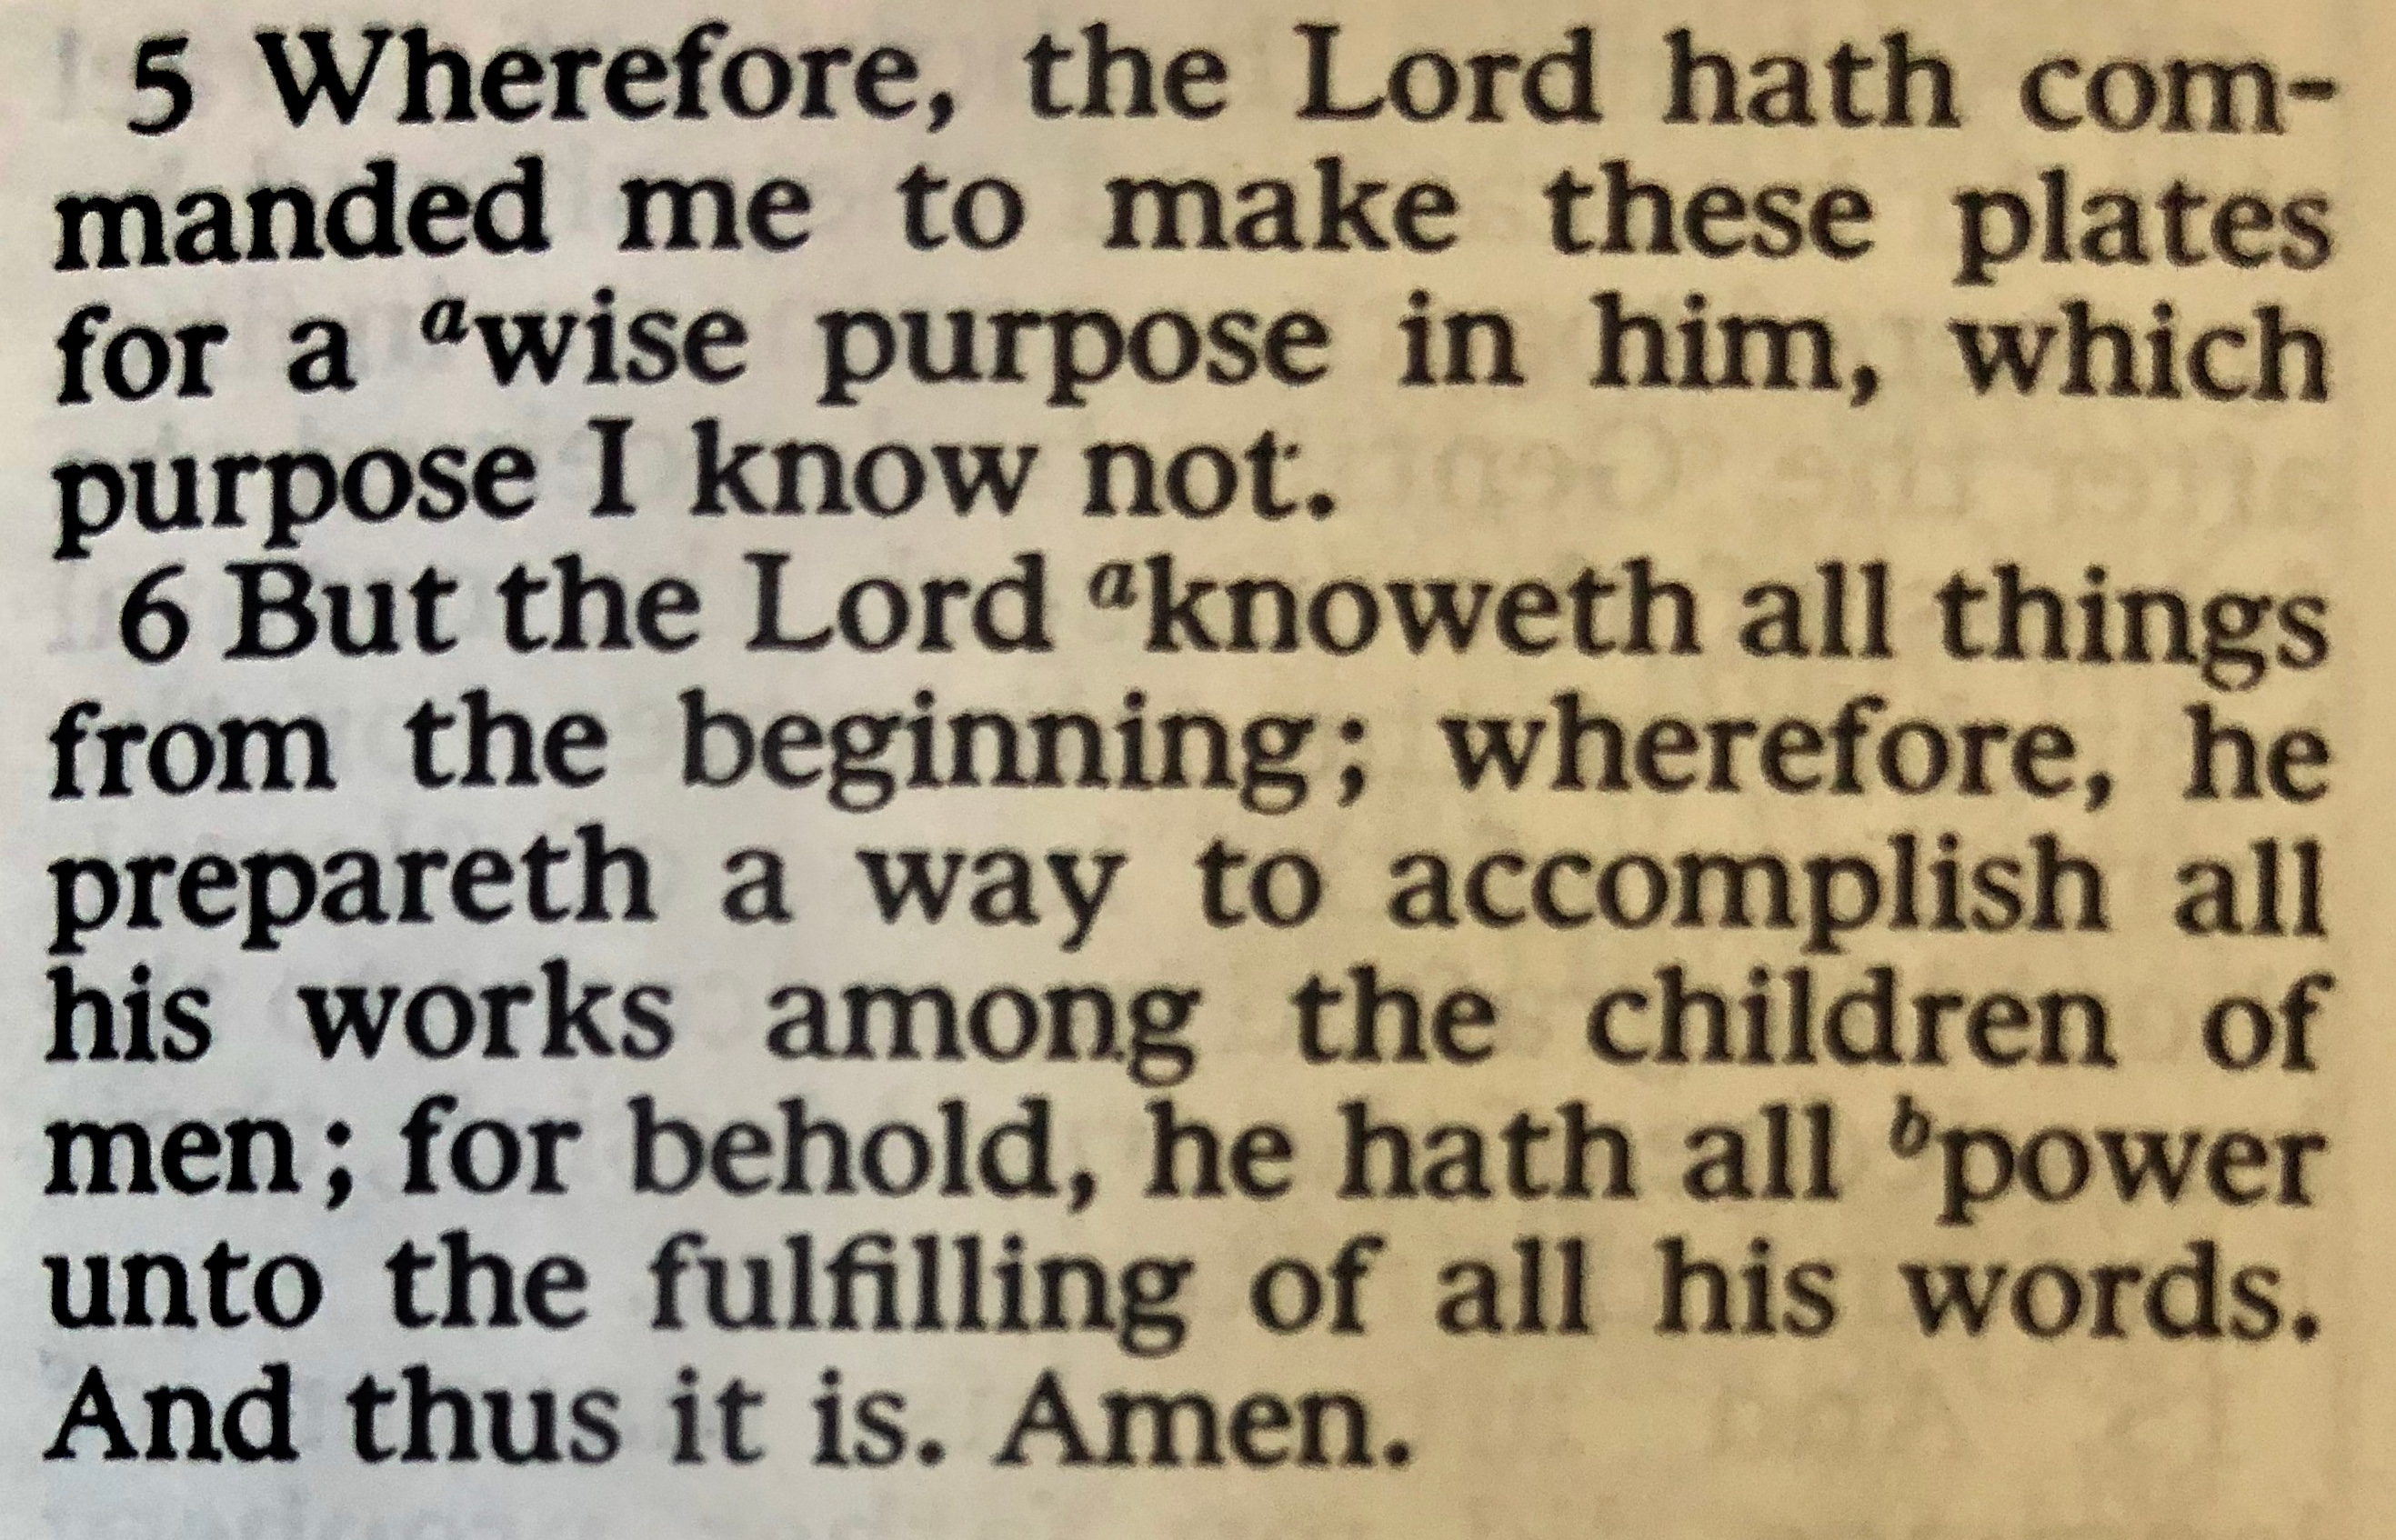
\includegraphics[width=.5\linewidth]{2018/images/know.jpg}
  \caption{God Knows All, 1 Nephi 9:5-6}
  \label{fig:knowledge}
\end{figure}

You know how they say time isn't predetermined. But god knows how events can unfold? 
But because we all have agency we could change things?

If that really were the case. The prophesies of the Bible and the BOM 
could have been easily foiled by people not doing what they said would happen.

What if Satan or Judas decided not to betray Christ? What would have happened? What
if Adam and Eve would have actually obeyed God's commandments? Would God have had to
find another way to have them ``sin"\footnote{transgress} and for us to find another
way to come to Earth?

God has a great Urim and Thummim, like a sea of glass. There's nothing He doens't
know. If that's the case? Which it has to be, because He's God. Then he knows
everything, God knows every decision a person will make. He has to know what will
happen in life. He can see into the future, and naturally the past. Anytime He
chooses to look at, God can look and see His children's doings.

\begin{displayquote}
Q. What is the sea of glass spoken of by John, 4th chapter, and 6th verse of the 
Revelation?

A. It is the earth, in its sanctified, immortal, and eternal 
state.\footnote{D\&C 77:1}
\end{displayquote}

And then again in the Doctrine and Covenants we find the following:

\begin{displayquote}
The angels do not reside on a planet like this earth;

But they reside in the presence of God, on a globe like a sea of glass and fire, 
where all things for their glory are manifest, past, present, and future, and are 
continually before the Lord.

The place where God resides is a great Urim and Thummim.

This earth, in its sanctified and immortal state, will be made like unto crystal and 
will be a Urim and Thummim to the inhabitants who dwell thereon, whereby all things 
pertaining to an inferior kingdom, or all kingdoms of a lower order, will be manifest 
to those who dwell on it; and this earth will be Christ's.

Then the white stone mentioned in Revelation 2:17, will become a Urim and Thummim to 
each individual who receives one, whereby things pertaining to a higher order of 
kingdoms will be made known;

And a white stone is given to each of those who come into the celestial kingdom, 
whereon is a new name written, which no man knoweth save he that receiveth it. The 
new name is the key word.\footnote{D\&C 130:6-11}
\end{displayquote}

For those who say that God isn't all knowing? They're wrong. He knows the past, the
present, and the future. There's no way He can't. For if God were to not know of
things to come, He wouldn't be perfect and would cease to be God.

At which point, do we have a chance? If God knows what we will do, and how we will
react to situations; He knows if we are damned before we even go back home. He knows
our doings and what will happen. There can be no doubt about that.

Jesus Christ suffered for the sins committed while here in  mortality, for all of
God's children. If that is the case, then were we not destined to commit such sins?
If Jesus suffered for all of our sins we would commit, so he can know what we went
through, then how do we even have agency? Such sins were placed upon us so we would
go through them, and I suppose learn from our mistakes. Jesus having bought our souls
so we become His begotten sons and daughters. There can be no agency in such a model.
It was all determiend before hand.
